% This is samplepaper.tex, a sample chapter demonstrating the
% LLNCS macro package for Springer Computer Science proceedings;
% Version 2.21 of 2022/01/12
%
\documentclass[runningheads]{llncs}
%
\usepackage[T1]{fontenc}
% T1 fonts will be used to generate the final print and online PDFs,
% so please use T1 fonts in your manuscript whenever possible.
% Other font encondings may result in incorrect characters.
%
\usepackage{graphicx}
\usepackage{subcaption}
\usepackage{url}
\usepackage[
    hidelinks
]{hyperref}
\usepackage{tikz}
\usepackage{pgfplots}
\usepackage{xurl}
\usepackage{pifont}
\pgfplotsset{compat=1.18} % Replace 1.18 with your current version if needed

% \setlength{\textfloatsep}{5pt}
% \setlength{\floatsep}{4pt}
% \setlength{\intextsep}{10pt}
% \setlength{\abovecaptionskip}{1pt}
% \setlength{\belowcaptionskip}{1pt}

% Used for displaying a sample figure. If possible, figure files should
% be included in EPS format.
%
% If you use the hyperref package, please uncomment the following two lines
% to display URLs in blue roman font according to Springer's eBook style:
%\usepackage{color}
%\renewcommand\UrlFont{\color{blue}\rmfamily}
%\urlstyle{rm}
%
\begin{document}

\title{Creation of a geo-historical address reference dataset from multiple sources}
%
\titlerunning{Geo-Historical Address Dataset}
% If the paper title is too long for the running head, you can set
% an abbreviated paper title here
%
\author{Charly Bernard\inst{1}\orcidID{0009-0003-8170-3671} \and
Nathalie Abadie\inst{2,3}\orcidID{0000-0001-8741-2398} \and
Bertrand Duménieu\inst{3}\orcidID{0000-0002-2517-2058}\and
Julien Perret\inst{3}\orcidID{0000-0002-0685-0730}}
%
\authorrunning{C. Bernard et al.}
% First names are abbreviated in the running head.
% If there are more than two authors, 'et al.' is used.
%
\institute{Univ Gustave Eiffel, Géodata Paris, IGN, LASTIG, F-77454 Marne-la-Vallée, \email{charly.bernard@ign.fr}, \email{nathalie-f.abadie@ign.fr, \email{julien.perret@ign.fr}}\\
\and
Centre de Recherches Historiques, École des Hautes Études en Sciences Sociales, Paris, \email{bertrand.dumenieu@ehess.fr}}
%
\maketitle              % typeset the header of the contribution
%
\begin{abstract}
Addresses are structured designations of places that are used by individuals to locate a precise destination - a building in a city, for example - with as little ambiguity as possible. These indirect spatial references encode spatial and hierarchical relationships between a large number of geographical entities, and taken in mass form a description of an area at different scales. In the case of old addresses, they can help to reconstruct the vanished structures of an area in great detail, and have a particularly powerful potential for the study of urban dynamics over the long term. The mass and heterogeneity of these objects make them difficult to use in computerised form, despite their abundance in digitised archives and structured data sources on the Web. In this article, we present an ontology for modelling addresses in all their diversity and for representing the temporal evolution of geographical entities. We also explain how and with what data we populate the ontology we have created.
\end{abstract}

% DEBUT DE L'ARTICLE
%
\section{Introduction}
\label{sect:intro}
The increasing availability of digitized archival sources and recent advances in information extraction approaches from texts and images, enabled by the rise of deep neural networks, now make it possible to exploit these sources to produce structured data on the various aspects of the past they describe.
Among the information that can be found in archival sources, addresses constitute a particularly important corpus, both in terms of volume and application potential.
First, they play a central role in various types of iconographic documents, such as city maps, as well as textual documents, including resident and business directories, civil status records, notarial documents, etc.
They are therefore available in large quantities, with a potentially significant overlap between sources.
Second, they reflect the evolution of cities, whose morphological and administrative changes they have accompanied over time.
For example, in Paris, several building numbering systems have successively been used since the Ancien Régime.
Finally, the main interest of addresses lies in their dual role as direct spatial references, when extracted from maps and described through coordinates, and indirect spatial references, when represented as textual information.
Indeed, having both representations makes it possible to geocode textual archival sources and locate the information they contain on the Earth's surface.

To structure and enhance the value of address-related information available in heterogeneous and fragmented forms within archival sources, we propose the construction of a geo-historical knowledge base on Parisian addresses.
The choice was made to focus exclusively on the French capital, as numerous sources are available for this city, covering a substantial period and representing addresses in various forms.
This knowledge base aims to structure the available knowledge on addresses, represent their temporal evolution, and describe the sources that mention them.
This article presents the ontology developed to represent the first two aspects of historical addresses extracted from archival sources.
We developed it following the methodology called \textit{Simplified Agile Methodology for Ontology Development} (SAMOD)~\cite{peroni_simplified_2017}, which consists in separating a complex modelling problem into smaller sub-problems, called modelets, which are easier to address, validate, and test.
A modelet starts with a natural language argumentation describing the sub-problem to be addressed, together with a glossary defining the key concepts and terms involved.
Each modelet is accompanied by a set of informal competency questions, also expressed in natural language, representing the questions that the knowledge base should be able to answer.
Each question is finally associated with a set of expected example answers, which are used to validate the modelet once implemented.
The modelling of geo-historical phenomena is complex and involves different themes from knowledge engineering; the SAMOD methodology makes it possible to identify and separate these themes in order to facilitate the design process.
Moreover, it enables rapid iterative cycles with regular evaluation of the ontology throughout its development.

This article is organized as follows.
We first present a state of the art on knowledge representation for addresses and the temporal evolution of geographic entities.
Then, we present the two modelets developed to represent addresses of all types and their evolution over time.
Finally, we populate these modelets using real-world data from various sources in order to assess their generality and their ability to effectively answer the competency questions initially defined.

\section{State of the art}
\label{sect:etat_art}
\subsection{What is an address?}
\label{subsect:def_adresses}

An address is primarily an indirect spatial reference, a structured statement that designates a location unambiguously~\cite{coetzee_towards_2011}.
Although the form and nature of what it designates vary depending on periods and locations,~\cite{morita_cheminement_1980} identifies two categories.
The administrative address, which only defines the position of a place, differs from the itinerary address, which describes a path through space.
"\textit{59 rue de Rivoli, 75001 Paris}" and "\textit{maison de la Belle-Jardinière, quai aux Fleurs, coin de la rue de la Cité}" are respectively examples of these two address categories.
An address is therefore a composite entity, made of spatial references organized into hierarchies and whose spatial relationships may be explicitly described~\cite{coetzee_towards_2011}.
These components are spatial landmarks, possibly informal, known and shared by the people using the address~\cite{dumedah_address_2021}.
In this article, an address is therefore defined as a structured statement describing a path within a spatial hierarchy, unambiguous within this hierarchy, composed of an ordered sequence of spatial landmarks whose conceptualization and designation are known and shared.

\subsection{Addressing systems in Paris since the 18\textsuperscript{th} century}
\label{subsect:histoire_adresses_paris}

\begin{figure}[ht]
     \centering
     \begin{subfigure}[b]{0.32\textwidth}
         \centering
         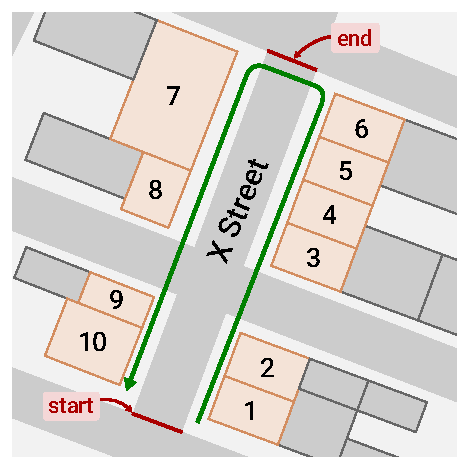
\includegraphics[width=\textwidth]{images/systemes_numerotation_paris_royal.pdf}
         \caption{Kreenfelt system}
         \label{fig:systemes_numerotation_paris_royal}
     \end{subfigure}
     \hfill
     \begin{subfigure}[b]{0.32\textwidth}
         \centering
         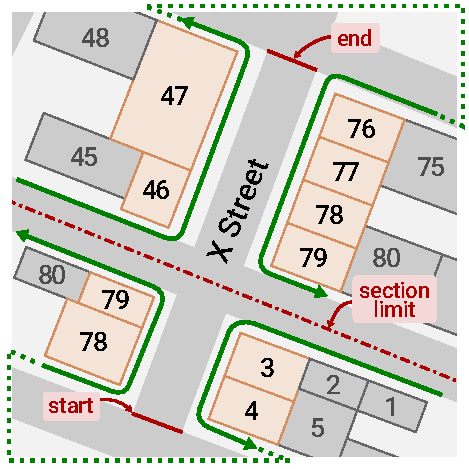
\includegraphics[width=\textwidth]{images/systemes_numerotation_paris_revolutionnaire.pdf}
         \caption{Revolutionary system}
         \label{fig:systemes_numerotation_paris_revolutionnaire}
     \end{subfigure}
     \hfill
     \begin{subfigure}[b]{0.32\textwidth}
         \centering
         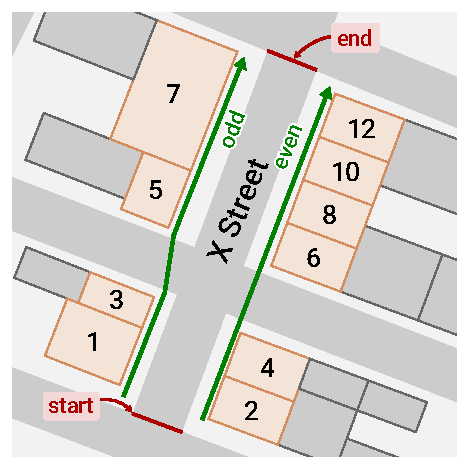
\includegraphics[width=\textwidth]{images/systemes_numerotation_paris_imperial.pdf}
         \caption{Imperial system}
         \label{fig:systemes_numerotation_paris_imperial}
     \end{subfigure}
     \caption{The three house numbering systems used in Paris. Green arrows indicate the numbering direction.}
     \label{fig:systemes_numerotation_paris}
\end{figure}

As in other European capitals, the numbering of houses in Paris appeared at the end of the 18\textsuperscript{th} century.
Until then, buildings were designated by a name, often a sign, sometimes complemented with additional information to disambiguate them~\cite{pronteau_les_1966}.
This designation was completed by relative positioning descriptions, such as "\textit{Maison du Pied de Griffon […] au coin oriental de la rue du Chantre, […] front sur la rue de Beauvais}"~\footnote{Adolphe Berty, Henri Legrand, Lazare-Maurice Tisserand, Théodore Vacquer, Camille Platon. Topographie historique du vieux Paris. Région du Louvre et des Tuileries, volume 1. Paris, imprimerie impériale édition, 1866.}.
Three numbering systems were successively introduced.

The first one, initiated privately, was proposed by Marin Kreenfelt, publisher of the \textit{Almanach de Paris}, in 1779~\cite{depaulis_vaugeois_2016}.
The entrances of buildings along the same street were numbered following a horseshoe-shaped path (Fig.~\ref{fig:systemes_numerotation_paris_royal}).
Probably little used in practice, these addresses were nevertheless included in the \textit{Almanach de Paris}.

The so-called \textit{sectionnaire} addressing system appeared during the French Revolution and did not last long.
Named after the subdivision of Paris into sections, it relied on this administrative division.
Created mainly for taxation purposes, this numbering system has never been fully reconstructed, as it relied on a general rule that was unevenly applied and on numerous undocumented local adaptations~\cite{fleury_concordance_1995,waquet_almanachs_2018}.
Numbering started at one end of a section and followed a path along the urban blocks composing it, with specific rules for each section (Fig.~\ref{fig:systemes_numerotation_paris_revolutionnaire}).

The third numbering system, still in use today, was created under the First French Empire.
It consists in numbering plots and buildings on both sides of each street in increasing order, with odd numbers on the left side and even numbers on the right side.
The starting point of a street, and therefore of its numbering, is in principle the end closest to the Seine (Fig.~\ref{fig:systemes_numerotation_paris_imperial}).

\subsection{Address modelling}
\label{subsect:representation_adresses}

Although the literature agrees on the general structure of an address as a set of landmarks connected by spatial relationships, postal addresses receive most attention due to their administrative importance.
Existing formal representation approaches mainly focus on this type of address, particularly for harmonization and standardization purposes within a country or region~\cite{coetzee_towards_2011,coetzee_what_2007,zandbergen_comparison_2008,borkar_automatically_2000}.

In geomatics, the ISO 19133 standard~\cite{iso_19133_2005} only addresses postal addresses.
Generic models remain poorly suited to more heterogeneous addressing systems.
For example, the relational model proposed by~\cite{davis_assessing_2007} decomposes addresses into geographic landmarks connected by spatial relationships, but with a systematic hierarchical structure: building, municipality, and region.
The \textit{locn} ontology\footnote{\url{http://www.w3.org/ns/locn}} follows a similar approach: its class \texttt{locn:Address} consists of an aggregation of \texttt{Literal} values rather than resources.
The types of landmarks are limited (street, administrative unit, etc.), and spatial relationships are not explicitly represented.

These proposals, designed for contemporary postal addresses, cannot be directly adapted to historical Parisian addresses~\cite{cura_historical_2018}.
For example, the address statement "\textit{situé sur le blv. de Clichy, dans la partie comprise entre la place Blanche et la rue Fontaine}" (\textit{located on Boulevard de Clichy, in the section between Place Blanche and Rue Fontaine}) cannot be represented using these models: no municipality is provided, more than one landmark of type Street is involved, and a spatial relationship is expressed in natural language through the term \textit{between}.
Finally, none of these models incorporates the fact that addresses evolve over time.

\subsection{Representing the temporal evolution of addresses}
\label{subsect:modelisation_evol_temp}

The representation of spatial dynamics has been investigated in several studies~\cite{hallot_identite_2012,carver_qualitative_1998,fan_time-based_2010,del_mondo_modegraphe_2011}.
These works share a central question: what defines the identity of a spatio-temporal entity?
For instance, when should an entity be considered created or disappeared?

\cite{hallot_identite_2012} proposes separating the identity of an entity from its physical reality.
Thus, a street is not created when it physically exists on the ground, but when it is planned.
The proposed temporal evolution model relies on the \textit{Identity Based Change} model~\cite{hornsby_identity-based_2000}.
The principle is based on alternating phases (or spatio-temporal states) during an entity's lifetime.
Changes are defined according to transitions between two phases.

\cite{hornsby_identity-based_2000} identifies three possible states for a geographic entity: existence, simple non-existence, and non-existence with a history;~\cite{hallot_identite_2012} proposes five.
With these approaches, entities can be considered as having potentially infinite lifetimes containing several existence states bounded by non-existence states.

Several approaches exist for constructing geo-historical graphs.
However, most of them are limited to homogeneous datasets with predefined temporal resolutions~\cite{armstrong_temporality_1988,dumenieu_systeme_2015,costes_vers_2016,bernard_ontologies_2018}.
They rely on detecting versions of geographic entities within independent sources, each describing a spatio-temporal state.
When differences exist between successive versions, changes are inferred.

This is the case of the TSN-Change ontology~\cite{bernard_ontologies_2018}, which traces the evolution of geographic entities (appearance, disappearance, name changes, etc.) within successive versions of the NUTS\footnote{Nomenclature of Territorial Units for Statistics, see \url{https://ec.europa.eu/eurostat/fr/web/nuts/background}}.
This nomenclature, published annually, is a hierarchical territorial subdivision of the European Economic Area.
The originality of this approach is that changes may involve several entities (merging, splitting, etc.) by decomposing them into elementary changes applied at the entity level.
\cite{bourel_graphes_2022} proposes the HHT (Historical Hierarchical Territory) ontology, which applies a similar approach to territories of the Ancien Régime.

To formally represent the temporal dimension of linked data, the W3C proposes the OWL-Time ontology, which allows temporal facts associated with resources to be expressed.
Based on Allen's temporal algebra, it allows events to be associated with instants or intervals and enables the temporal ordering of facts~\cite{pan_time_2006}.

\section{Proposition}
\label{sect:proposition}
\subsection{Addresses}

\begin{figure}[ht]
    \centering
    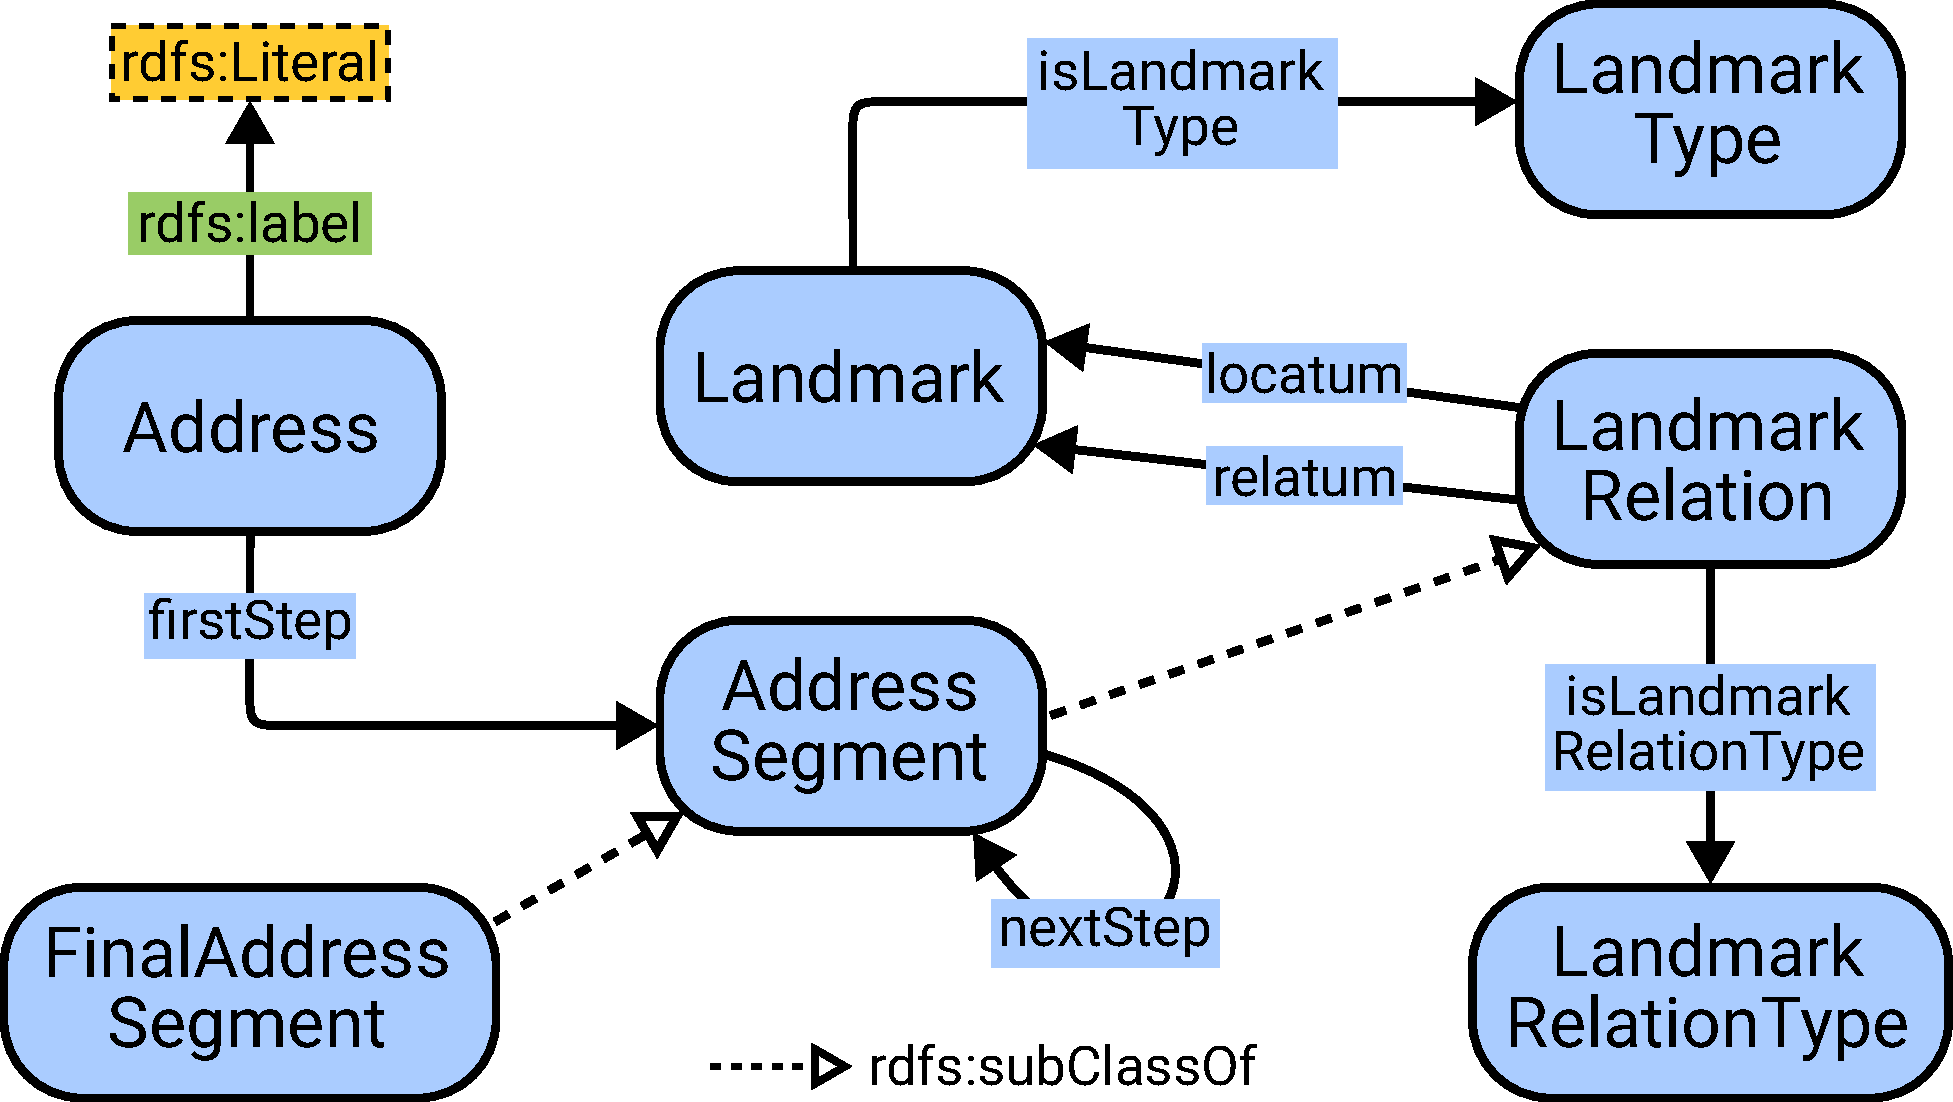
\includegraphics[width=0.8\textwidth]{images/address_ont.pdf}
    \caption{Simplified representation of the ontology.}
    \label{fig:address_ont}
\end{figure}

\begin{figure}[ht]
    \centering
    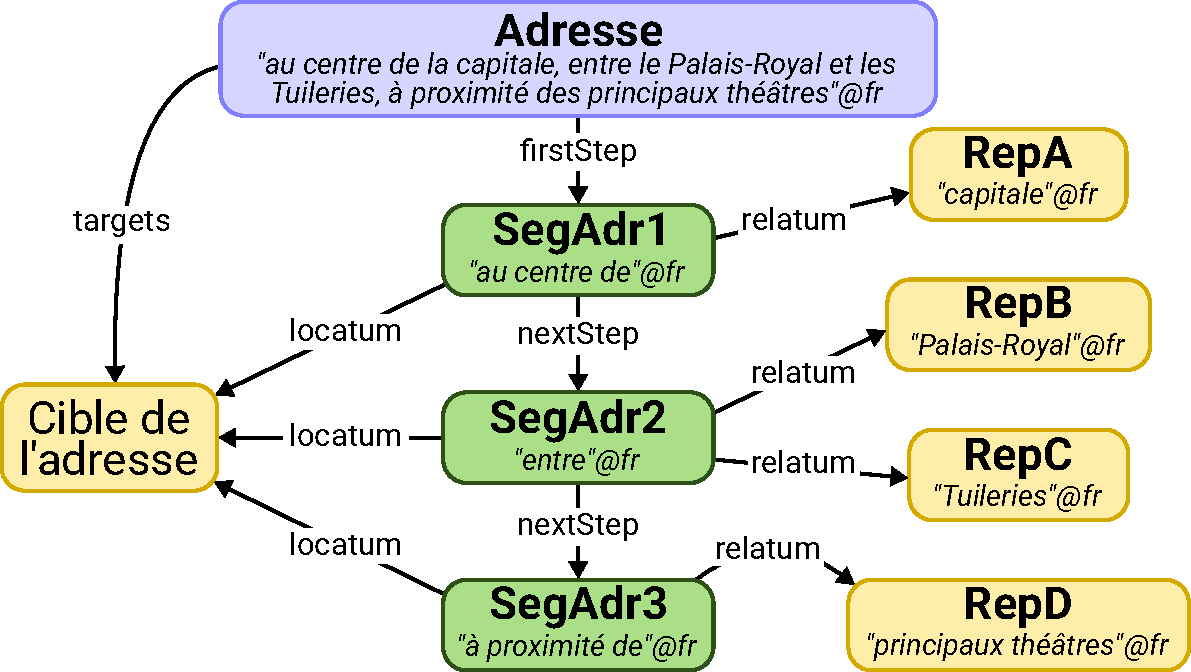
\includegraphics[width=0.9\textwidth]{images/exemple_modelisation_adresse.pdf}
    \caption{Example of address modelling.}
    \label{fig:exemple_modelisation_adresse}
\end{figure}

In this modelet\footnote{\texttt{https://github.com/charlybernard/phd-ontologie}}, an address is composed of references to spatial landmarks, connected by spatial relationships, which together point to a target location to which geographic coordinates can be associated.
Therefore, we selected the following competency questions:
(1) what are the addresses listed along a given street?
(2) what are the coordinates corresponding to the target of a given address?
(3) what are the addresses located within a given area?

The ontology, presented in Figure~\ref{fig:address_ont}, contains three concepts:
\begin{itemize}
    \item the address (\texttt{Address}), corresponding to the statement describing a location;
    \item the address segment (\texttt{AddressSegment}), a subclass of~\texttt{LandmarkRelation}, describing a relation between landmarks involved in an address. The nature of this relation is defined by~\texttt{LandmarkRelationType};
    \item the landmark (\texttt{Landmark}), describing a geographic entity. \texttt{LandmarkType} defines its nature (e.g., administrative unit, street, house number, building, etc.).
\end{itemize}

The location designated by an address is represented as a~\texttt{Landmark}, while the sequence of geographic references composing the address is represented through resources of type~\texttt{AddressSegment} which is a subclass of~\texttt{LandmarkRelation}, each segment represents a typed relation between two landmarks.

A resource of type~\texttt{Address} is linked through the property~\texttt{firstStep} to the first resource of type~\texttt{AddressSegment}. Each segment is then linked through the property~\texttt{nextStep} to the following segment, and so on. The type of relation represented by each segment is specified using~\texttt{LandmarkRelationType}. To represent the end of this sequence, the last resource is typed as~\texttt{FinalAddressSegment}, a subclass of~\texttt{AddressSegment}.

A resource of type~\texttt{AddressSegment} describes a step in the path linking a landmark, called the \textit{locatum}, to one or more landmarks called \textit{relatum}~\cite{tenbrink_model_2011}.
Generally, the locatum corresponds to the target of the address, as each step of the path aims to provide additional information about its location.
The example presented in Figure~\ref{fig:exemple_modelisation_adresse} illustrates this principle.
The address points to an unknown landmark and has a label that can be divided into three parts:
"\textit{in the centre of the capital}",
"\textit{between the Palais-Royal and the Tuileries}",
and
"\textit{near the main theatres}".
There are three address segments and four references to geographic landmarks.

\subsection{Temporal evolution}
\label{sect:prop_evolution_temporelle}

\begin{figure}[ht]
\begin{center}
 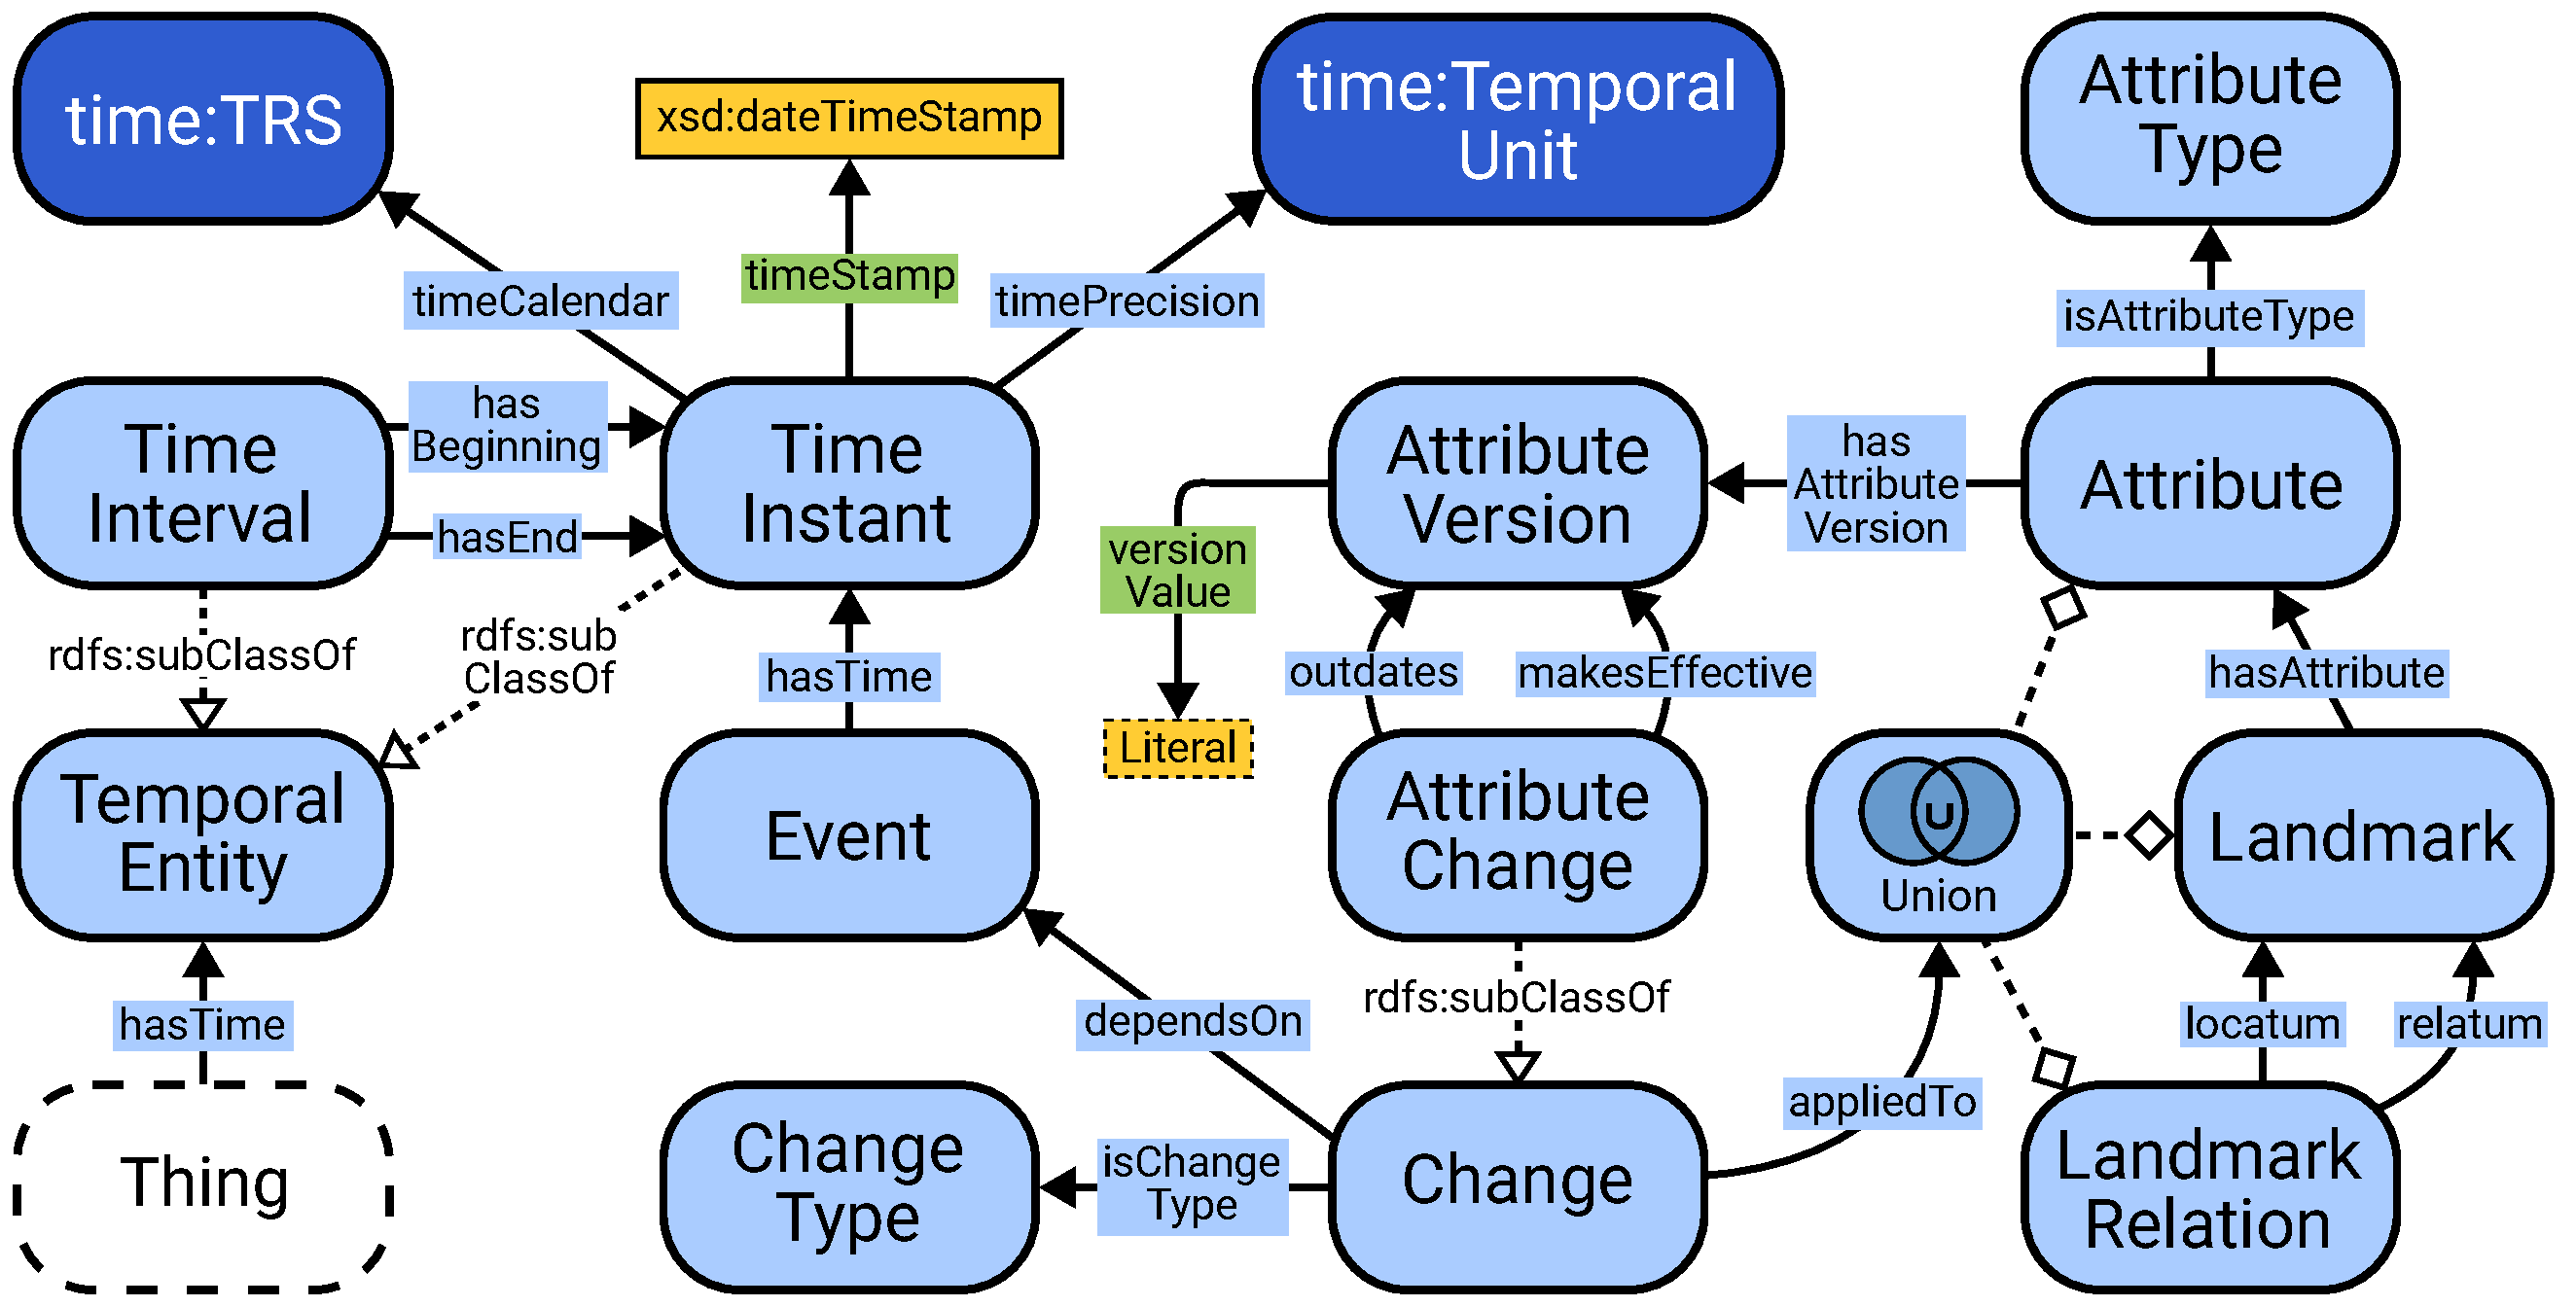
\includegraphics[width=\textwidth]{images/events_ont.pdf}
 \caption[]{Representation of the ontology for the temporal evolution of geographic landmarks\footnotemark.} 
\label{fig:events_ont}
\end{center}
\end{figure}

\footnotetext{The element linked to the class \texttt{Change} through the predicate \texttt{appliedTo} describes the union of \texttt{Attribute} and \texttt{Landmark}.}

For this modelet, we identified the following competency questions:
(1) which streets exist at a given time?
(2) over which temporal interval(s) is a given address name valid?
(3) what is the history of a landmark? In other words, which events are associated with it?
(4) which states and events are missing from the history of an address?

Two main requirements emerge from these competency questions:
the ability to retrieve the state of geographic landmarks at any given time, and the representation of events that have affected geographic landmarks and their properties.

For the second aspect, we draw inspiration from the work of~\cite{bernard_ontologies_2018} by decomposing events into elementary changes that explicitly describe the transition between two versions.
In addition to applying changes to landmarks, we chose to associate changes with landmark attributes.
This makes it possible to determine the evolution of a specific attribute.
For this purpose, a property associated with a landmark is represented through a resource of type~\texttt{Attribute}, to which versions are attached.
Whenever a change affects a landmark or one of its attributes, it is represented by a resource of type~\texttt{Change}, which specifies the resource affected by the change.

\cite{bernard_ontologies_2018} studies the evolution of entities through \textit{snapshots}, meaning that changes describe the evolution between two successive versions of an entity, even when no difference exists between them.
This approach is discrete, whereas our objective is to assign each entity its own validity time in order to describe the state of the territory at any given moment, which is enabled by our modelling.

Figure~\ref{fig:events_ont} presents the four main concepts of the ontology:

\begin{enumerate}
    \item the change (\texttt{Change}), which describes an elementary operation of an event. If it applies to a geographic landmark, the change is a \texttt{LandmarkChange}; if it applies to an attribute (such as the name of a street), it is an \texttt{AttributeChange}. \texttt{ChangeType} defines its type (e.g., appearance or disappearance of a landmark);
    \item the attribute (\texttt{Attribute}), whose type is defined by \texttt{AttributeType};
    \item the attribute version (\texttt{AttributeVersion}).
\end{enumerate}

\begin{figure}[ht]
\begin{center}
 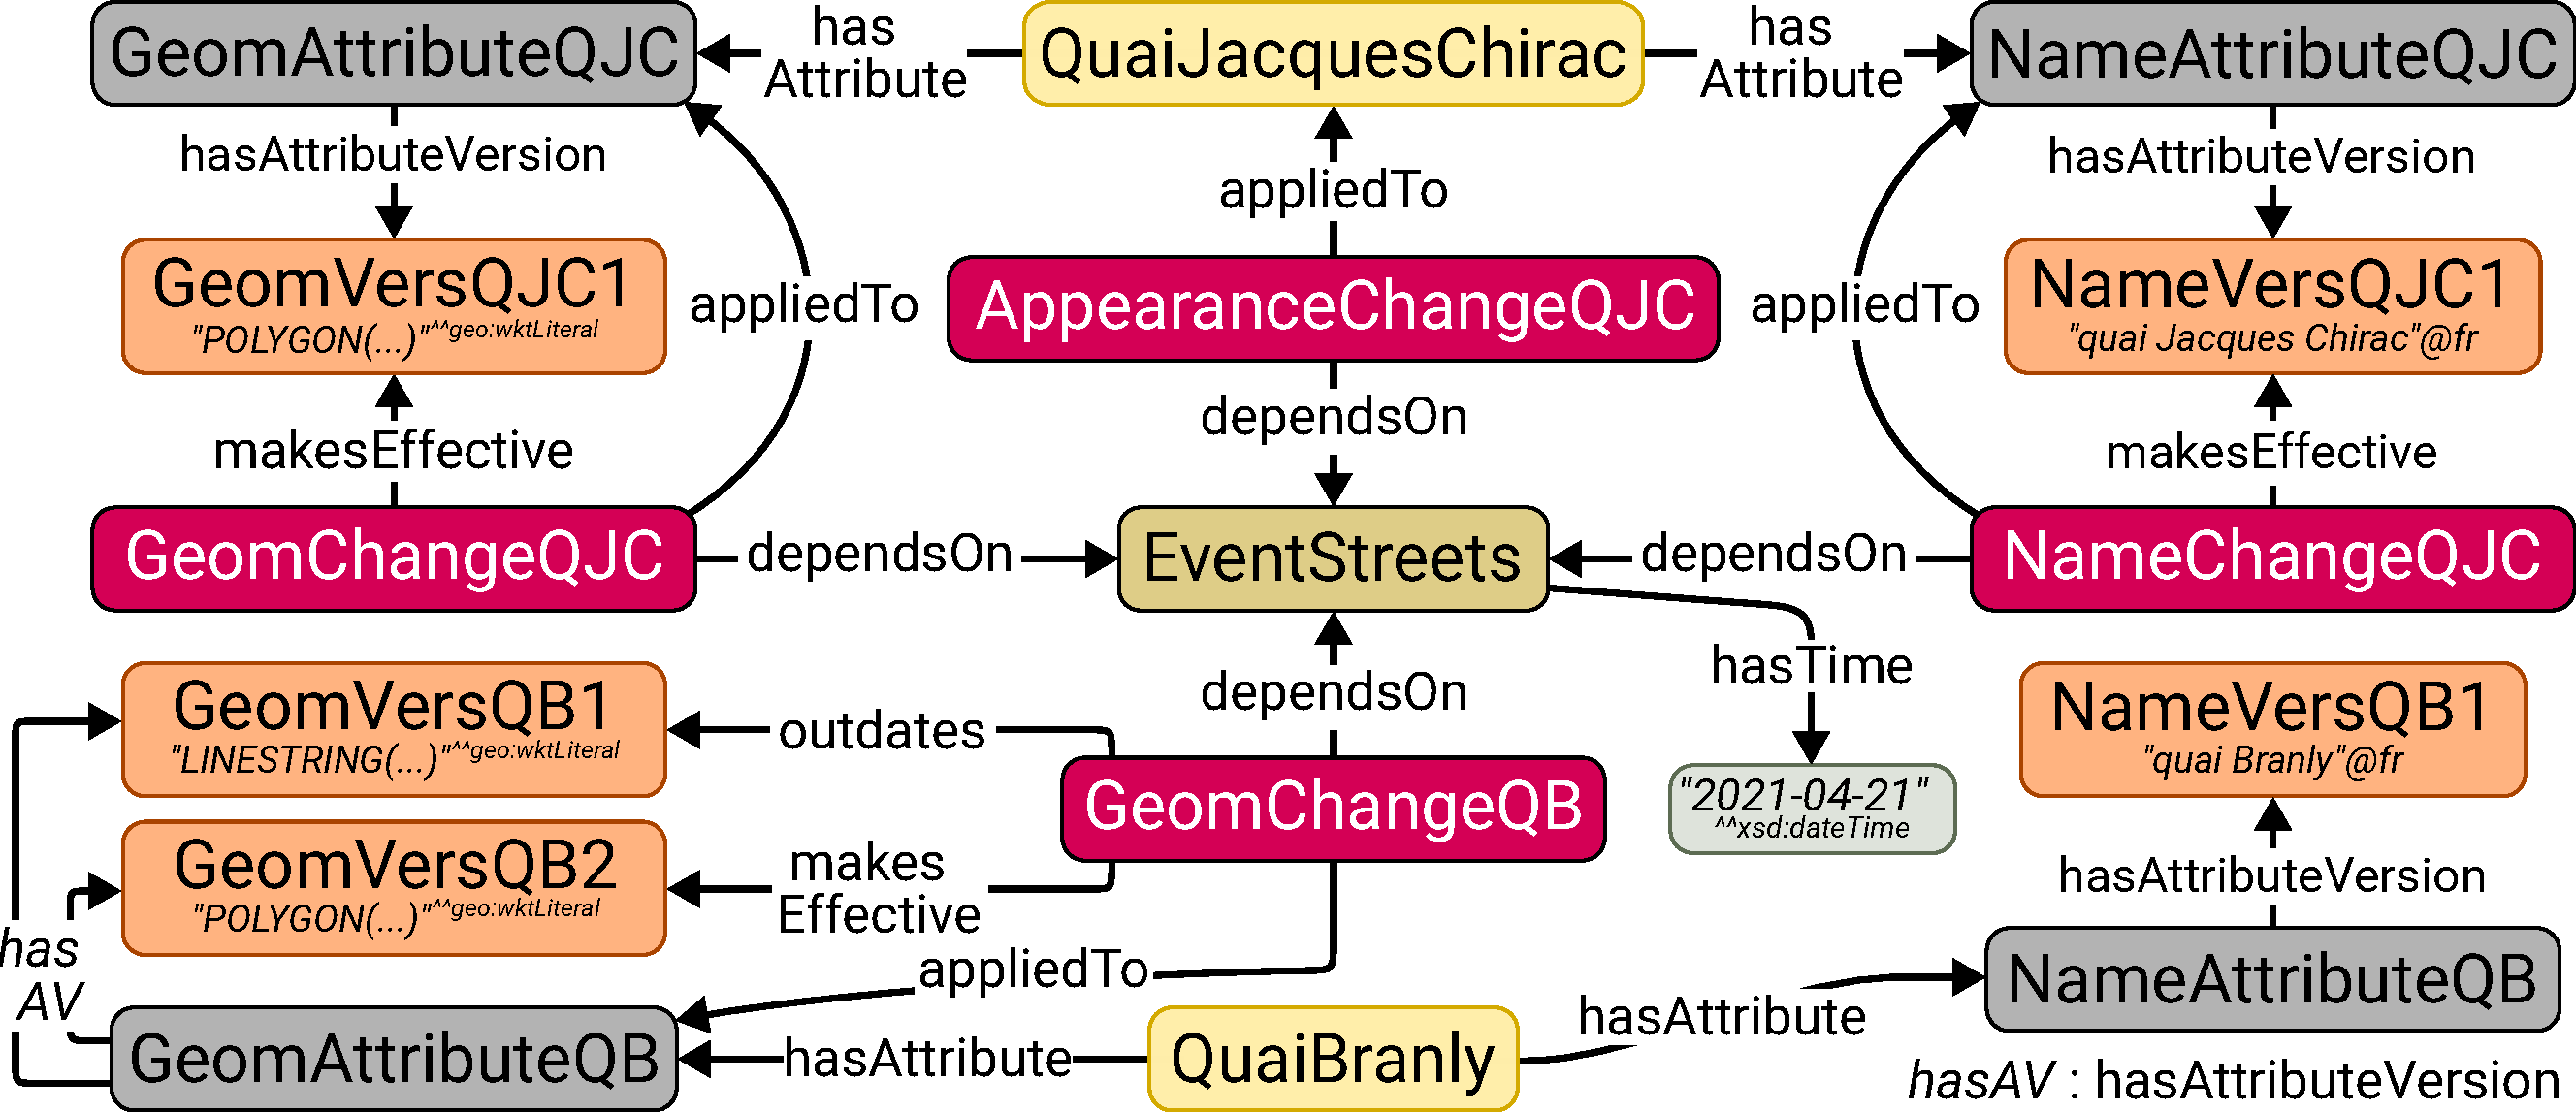
\includegraphics[width=\textwidth]{images/exemple_modelisation_temporelle.pdf}
 \caption{Example of modelling the joint evolution of two streets: creation of \textit{quai Jacques Chirac} through the subdivision of \textit{quai Branly}.}
 \label{fig:exemple_modelisation_temporelle}
\end{center}
\end{figure}

With this modelling, modifications involving one or several geographic entities can be decomposed into elementary changes.
Consider the event "creation of quai Jacques Chirac from a portion of quai Branly on April 21, 2021".
As represented in Figure~\ref{fig:exemple_modelisation_temporelle}, it can be divided into several changes:

\begin{itemize}
    \item appearance of the landmark \texttt{QuaiJacquesChirac};
    \item creation of a new version of \texttt{NameAttributeQJC}, a name attribute, for which no previous version exists;
    \item creation of a new version of \texttt{GeomAttributeQJC}, a geometry attribute, also without a previous version;
    \item creation of a new version of \texttt{GeomAttributeQB}, the geometry attribute of quai Branly, whose previous version corresponded to the spatial extent of the quay from Place de la Résistance to Pont d'Iéna.
\end{itemize}

\section{Implementation and evaluation}
\label{sect:implementation}
The consistency of the proposed ontologies and their compliance with ontology design best practices were verified using the HermiT reasoner integrated into Protégé\footnote{\url{http://protege.stanford.edu/}}~\cite{musen_protege_2015}, as well as the OOPS! tool\footnote{\url{https://oops.linkeddata.es/}}~\cite{poveda-villalon_oops_2014}.

\subsection{Population and validation of the address ontology}

The address ontology is also evaluated by populating it with three address datasets for Paris: two contemporary sources, OpenStreetMap (OSM) and the French National Address Database (BAN), and one historical source consisting of addresses extracted from the nineteenth-century Paris trade directories~\cite{abadie_benchmark_2022}. The integration process for these sources comprises three steps: (1) identifying the landmarks and spatial relationships composing the addresses, (2) structuring each address according to the proposed model, and (3) linking addresses referring to the same target.

\begin{table}[htbp]
    \centering
    \begin{tabular}{|l|l|l|l|l|l|l|}
    \hline
        num & rep & street\_name & postcode & city & lon & lat \\ \hline
        5 & & Boulevard Saint-Martin & 75003 & Paris 3rd & 2.361407 & 48.867933 \\
        134 & & Boulevard Raspail & 75006 & Paris 6th & 2.309998 & 48.86011 \\
        4 & & Rue Regnard & 75006 & Paris 6th & 2.338073 & 48.849885 \\
        48 & bis & Rue de Rivoli & 75004 & Paris 4th & 2.35448 & 48.85690 \\ \hline
    \end{tabular}
    \caption{Extract from a BAN file for the city of Paris. The address locations (provided by the \texttt{lat} and \texttt{lon} fields) in the BAN do not follow a single positioning rule. For each address, the method used to determine the location is specified (postal delivery point, entrance door, parcel centroid, etc.).}
    \label{tab:ban_sample}
\end{table}

The first step is straightforward for OSM and BAN data, which consist of postal addresses whose components are already separated. Structuring the historical addresses extracted from the Paris trade directories, which are more organic in nature (Figure~\ref{fig:exemple_modelisation_adresse}), is considerably more difficult, and off-the-shelf parsing tools such as LibPostal\footnote{\url{https://github.com/openvenues/libpostal}} fail to process them correctly. We therefore structured these addresses manually. The data from each source are then formatted as CSV or JSON, possibly after minor restructuring. For example, the BAN data (Table~\ref{tab:ban_sample}) are adapted by creating a \texttt{house\_number} field that concatenates the \texttt{num} and \texttt{rep} fields.

A mapping is defined for each source to specify how addresses should be converted into RDF according to the proposed ontology. This mapping identifies the landmarks and spatial relationships involved. We use Ontotext Refine\footnote{\url{https://www.ontotext.com/products/ontotext-refine/}} to construct these addresses. For a BAN file, the mapping creates nine resources: one \texttt{Address}, four \texttt{AddressSegment} resources, and four \texttt{Landmark} resources (\texttt{HouseNumber}, \texttt{Thoroughfare}, \texttt{PostalCode}, and \texttt{City}). The resulting graph contains duplicate landmark resources because addresses are created independently. For example, addresses located along the same street each generate a distinct resource describing that street. The final step therefore consists in removing duplicates using SPARQL queries: landmarks of the same type, having similar names and equivalent spatial relationships, are merged.

Once populated, we verified that the ontology can answer the predefined competency questions, translated into SPARQL queries. For example, the query retrieving all addresses targeting a place located along a given street (here, Rue du Dahomey) returns 16 addresses together with their coordinates, which are mapped in Figure~\ref{fig:localisation_adresses_rue_dahomey_paris}.

\begin{figure}[ht]
\begin{center}
 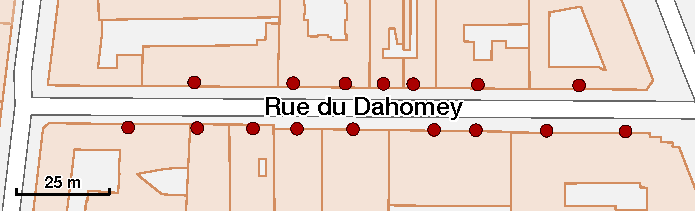
\includegraphics[width=0.85\textwidth]{images/localisation_adresses_rue_dahomey_paris.pdf}
 \caption{Location of addresses whose target is located along Rue du Dahomey.}
 \label{fig:localisation_adresses_rue_dahomey_paris}
\end{center}
\end{figure}

\subsection{Population and validation of the temporal evolution ontology}

To populate the ontology describing the temporal evolution of geographic landmarks, we used Wikidata data on the streets of Paris. These data include information such as creation dates and the successive official names of streets, together with their start and end dates of validity. From these data, we create \texttt{Thoroughfare} landmarks, name attributes together with their successive versions, and the corresponding changes.

Wikidata describes the successive states of streets. Therefore, for each state, we create two changes indicating respectively the beginning and the end of the state's validity. As a consequence, all changes are initially created independently and may therefore be duplicated. They must subsequently be merged using SPARQL queries.

Only a subset of the competency questions presented in Section~\ref{sect:prop_evolution_temporelle} could be translated into SPARQL queries, since this dataset is limited to the historical evolution of streets.

The history of a geographic entity can be reconstructed either by querying all the changes applied to the entity or by rebuilding its successive versions from the available changes, as illustrated in Figure~\ref{fig:evolution_place_nation}. Here, the states are inferred from the recorded events and may differ depending on which events are taken into account.

\begin{figure}
\begin{center}
 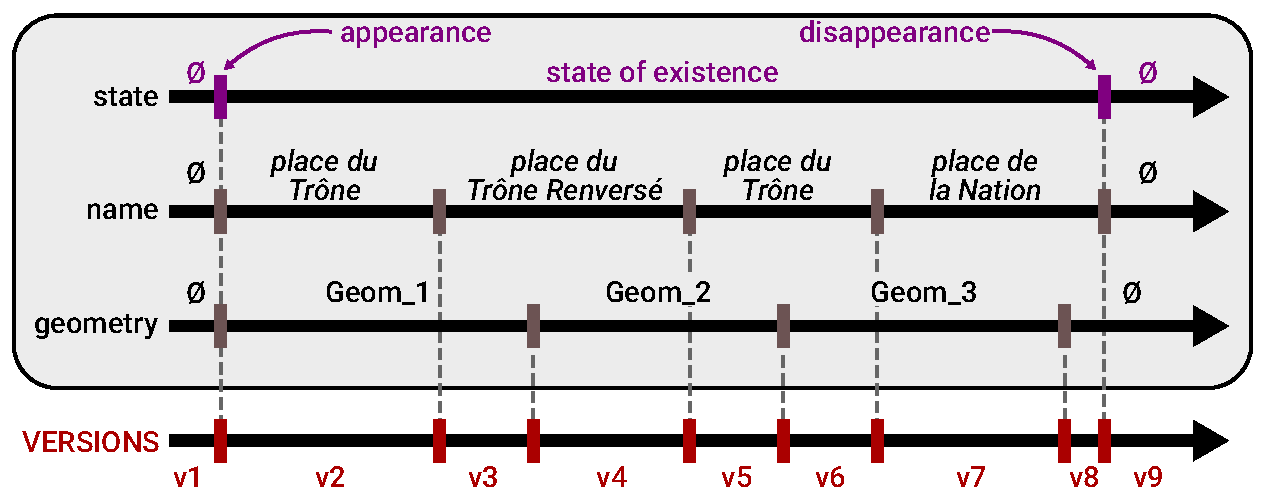
\includegraphics[width=\textwidth]{images/evolution_place_nation.pdf}
 \caption{Reconstruction of the successive states of Place de la Nation from the recorded changes.}
 \label{fig:evolution_place_nation}
\end{center}
\end{figure}

\section{Discussion}
\label{sect:discussion}
In this paper, we presented two ontologies: one for modelling the diversity of addresses and another for representing the temporal evolution of the geographic landmarks that compose them. Together, they support the incremental construction of a geo-historical knowledge graph from fragmentary data. However, several limitations remain and will need to be addressed in future work. First, temporal values associated with events are currently assumed to be known and precise. Since uncertainty is an inherent characteristic of historical data, future developments should explicitly account for temporal imprecision. Second, the ontology does not yet support the temporal evolution of relationships, particularly the spatial relationships linking geographic landmarks.

Following the SAMOD methodology, one remaining ontology module still needs to be developed to represent data sources and the assertions they contain. This module will enable the knowledge graph to be populated from heterogeneous information fragments while also managing conflicts between potentially contradictory sources.

Finally, to further validate the proposed ontologies, we plan to populate them with a wider variety of datasets covering Paris. These include historical cartographic sources providing \textit{snapshot}-like geometries, such as the Verniquet and Jacoubet atlases; structured datasets covering different time periods, such as the \textit{Dénominations caduques des voies de Paris}\footnote{\url{https://opendata.paris.fr/}} and the French National Address Database (BAN)\footnote{\url{https://www.data.gouv.fr/fr/datasets/base-adresse-nationale/}}; and unstructured historical sources, such as historical trade directories and textual descriptions of street histories available on Wikipedia. The resulting geo-historical knowledge graph is intended to support the development of a historical geocoding tool capable of locating historical addresses in both space and time within the city of Paris.

\bibliographystyle{splncs04}
\bibliography{references}

\end{document}